\part{Introduction}
\addto{\captionsenglish}{% Making babel aware of special titles
  \renewcommand{\mtctitle}{Another Title}
}

\startcontents[chapters]
\printmyminitoc{
}


\chapter{Exoplanet detection and characterization using high contrast imaging}
Generally describes what are the advances made in exoplanet detection and characterization
cover those areas where spectra and characterizations are available
\section{Direct exoplanet detections and characterizations}

\chapter{Introduction to machine learning algorithms}
\label{chap:III.2}
Machine learning (ML) algorithms are considered a class of algorithms that learn intrinsic relationships in the data in order to predict specified outputs that depend on these intrinsic relationships in the data.
These relationships between specified outputs and the data can be learned in one of three well known ways,
\begin{enumerate}
    \item \textbf{Unsupervised learning:} where the ML algorithm exploits the intrinsic relationships within data to learn features and use such features to derive the desired output without any external interventions.
    Algorithms in this class are typically used with data where intrinsic relationships in the data are not well established a priory.
    %might be very useful to derive the desired output.
    For example, unsupervised K nearest neighbors algorithms are frequently used to identify clusters within the data that might indicate data grouping which is not easily understood such as looking for data that could be analyzed for transients \citep[e.g][]{2022AleoTransients}, or finding cluster groups in open cluster data \citep[e.g][]{2022cluster}.
    Within Astronomy principal component analysis is a very well known unsupervised ML algorithm typically used in identifying structures in the data that can be discarded.
    Unsupervised ML algorithms are particularly useful for instance in anomaly detection \cite{2023EJASPanomaly}.
    Selecting parameters in the data which will enable other ML algorithms to perform better on the data can also be achieved through unsupervised methods \cite{2023PatRe.14209676H}.
    Principal component analysis is particularly useful in detecting such useful parameters in the data and has been proposed for instance to detect oceans in exoplanet data \citep[e.g][]{2022RyanOCeans}.
    Within the field of high contrast imaging unsupervised ML algorithms have been used in the package \citep[PACO,][]{2023Chomez} and \citep[VIP, ][]{2023Christiaens} also provides this capability. 
    \item \textbf{Supervised learning:} where the algorithm is shown multiple combinations of relationships between desired outputs for a set of inputs over multiple times and thus `trained' to learn the relationship between the input and the output.
    Algorithms in this class are typically used when there is a large amount of labelled data and typically when the relationship between the desired output and input is well known.
    This class of algorithms are also very effective when the desired output represents a non-linear combination of inputs for instance inferring for instance that a picture contains a cat from the presence of whiskers, eyes, nose etc in the picture.
    A famous example of such supervised learning was the handwritten digit recognition where a ML algorithm is trained to recognize handwritten digits in the US postal system and has now been improved on with the latest advances in supervised learning \cite{kussul2004improved}.
    This class comprises of a large set of algorithms spanning from \citep[neural networks,][]{gurney1997introduction} to \citep[random forests,][]{breiman2001random} to modern day \citep[transformers,][]{vaswani2017attention}.
    The advantage of supervised algorithms is that they are able to learn many complex relationships in the data. 
    However, the intrinsic problems of this class is that it requires a large amount of data, where this is relationship is well known.
    Supervised learning schemes suffer from the significant problem of learning the unintended relationships in the data when it is not trained appropriately or it is tested with wrong data.
    In the same example as before, if the algorithm is trained to recognize only cats and we present a dog, it will indeed mis-identify a dog as a cat because of the similarity of the features.
    It is also possible that while learning the possible relationships between the images and the presence of a cat, the algorithm learns that the any indoor setting is a picture of a cat because of our data contained only indoor cats.
    \end{enumerate}
In this thesis, we focused only on supervised learning for the following reasons,
\begin{itemize}
    \item the goal of the my thesis is to derive the presence of an exoplanet given certain discriminatory conditions in my input such as the spectral features corresponding to the planet.
    Such `conditions' are typically called features in ML algorithm training.
    \item a good prior knowledge of such a relationship exists (and is proven using non-ML algorithms such as cross correlation) and a large number of similar datasets exist for me to train a supervised algorithm,
    \item and finally, supervised algorithms allow us to specify the kind of output we need in astrophysics rather than relying on pre-existing relationships within data.
\end{itemize}
The act of producing data pairs of input and desired output is known as `labelling' and is typically carried out before training or testing any algorithms.
The desired outputs which are the result of a specific input combination are respectively called the `label' and the `data'. 
The data, thus, consists of multiple intrinsic parameters which as stated before are called features and the ML algorithm will typically learn which of these features are important for the desired output.
In our case the desired output is whether an extracted spectrum is that of a planet and the features that we use to arrive at this result is the spectral absorption bands.

\section{Types of supervised algorithms}
\label{sec:classifcation and regression}
Supervised learning can be further categorized based on the type of desired output as a regression and classification problems.

\textbf{Regression:} 
When the output of the supervised learning algorithm is a floating point number such as the distance or the intensity then such problems are called regression problems. 
Regression problems are usually adopted when the ML algorithm is meant to produce an unbounded output (except by the intrinsic rules set by the case itself for instance distance cannot be negative). 
This is also useful when we don't know precisely what the expected output is for a specific input, for instance distance between two points in an image can have a infinite values and this changes from each input to another.
Within regression problems, we also have types of regression based on the bounds of the output parameter.
For instance if the bounds are between $0$ and $1$, such regression is known as logistic regression.
The fundamental limitation of the regression problem is that there is an intrinsic uncertainty in the result. 
If sufficient information is presented then this uncertainty can be constrained to be within a few percent.
However, in some cases the output itself is constrained to be within a few finite values. 
Such class of problems are called classification problems.
Astronomy has many regression problems where for example galaxy photometric parameters have been estimated using machine learning algorithms \cite{2022YinAEparameter}.
Time series forecasting in astronomy has also been framed as regression problem \cite{2018Modred}.

\textbf{Classification:}
Classification problems are where the output classes are already well known, for example when the input is a set of words the machine learning algorithms classifies these words in to the emotions they are associated with such as happiness, anger etc. 
Classifiers have been also used to predict for instance liver lesions \cite{2023Nanda} in medical imaging. 
In astronomy classifiers have been used to differentiate between stars, blazars and quasars \cite{2023Zhao} in WISE data.
They have also been famously used to morphologically classify galaxies in the SDSS DR17 \cite{2019MNRASFischer}.
Classifiers in exoplanet direct imaging have been used by \citep[SODINN, ][]{2018Gomez} and \citep[NA-SODINN][]{2023Carlito}.
While classification has the adavantage of knowing the precise set of values that needs to be predicted, it also has the problem of the classes themselves being categorical.
For instance, \citep[SODINN, ][]{2018Gomez} wants the class of $C^{+}$, which is not a numerical value.
Typical classifiers work with either neural networks or ensemble classifiers such as \citep[Random Forests, ][]{breiman2001random} that produce floating point outputs.
In order to convert these numerical values we do the following two step process,
\begin{enumerate}
    \item For an $n$ class classification We first create an $n-1$ sized array.
    Therefore, a $10$ class classifier will output an $9$ element array, 
    \item we then encode the classes using routines such as \citep[One hot encoding][]{harris2010digital} that allows to convert a categorical class into a encoded value, where each position in the array is encoded as a $1$ for its corresponding class.
    The case where all array elements are $0$ also corresponds to a class, thereby covering all classes
\end{enumerate}
This encoded data is now considered as the value that the ML algorithm needs to predict.
Thus the ML algorithm will predict a value for each position in this array, typically values will range between $0$ and $1$ for each position following the sigmoid function.
Each value is thus a probability of the class and thus the class that the algorithm predicts would be the position with the highest probability.
We also at time provide a threshold above which the highest probability is accepted and this becomes the decision boundary of the classifier.

While classifiers are some of the most widely used type of supervised algorithms, they also suffer from the issue where some classes are better represented than the others. 
They also require large number of labelled examples.
These examples have to provide adequate representation of each of the classes, the noise distribution of the noise in each of these class samples should also mimic realistic noise in the data and finally, the samples themselves have to be representative of the data that the algorithm is expected to realistically classify.
In order to meet these requirements, we adopt training methodologies to adequately `train' an algorithm and then adopt specific testing methodologies to realistically estimate the performance of such algorithms. 
These are common for all supervised algorithms, sometimes the testing methodology can still be adopted for unsupervised algorithms as well.
In this thesis when we say ML algorithms it is taken to mean supervised ML algorithms.
\section{Training and testing supervised algorithms}
When generating labels for supervised data there is an intrinsic relationship between the data and its corresponding label.
This relationship could be either linear or non-linear and can thus be mapped to generate the output $y$ from input data $x$ as,
\begin{equation}
    y = f(x)
    \label{eq:y=fx}
\end{equation}
where $f(x)$ represents a function mapping $x$ to $y$
A special case of this linear relationship would be a straight line where $y$ and $x$ are related by its slope $m$ and interecept $c$,
\begin{equation}
    y =  m x + c
    \label{eq:line}
\end{equation}
ML algorithms have been trained in various contexts to derive such relationships between $x$ and $y$ based on large amount of data.
Such a process by which the ML algorithm is tuned to mimic $f(.)$ is called `training'.

Training requires sufficient number of data points that correspond to the expected output $y$. 
The function $f(.)$ is represented by the parameters of the ML algorithm which allow it to produce $y$  given $x$. 
These parameters differ based on the ML algorithm in question, their tuning will be explained in detail in the section corresponding to those class of algorithms.
In order to train an algorithms, we must first prepare the data so that this training is adequate, but not so targeted that the trained `model' can no longer generalize to new data.
The data usually has two characteristic elements, the data or $x$ which consists of images or spectra and the desired result or target output $y$ which is in our case whether the input corresponds to that of a warm Jupiter or not.
In this case it is important that ML algorithm learns the generalized features in the data corresponding to the presence of a warm Jupiter but avoids learning noise structures present only along with the warm Jupiter which would be a systematic of data acquisition.
Typically, this is solved with acquiring data with enough different types of systematics which would convince our model to learn only the common features, since this is not possible to achieve in practise we try to generate large amounts of data and try to evaluate how generalized the model is.
In order to ensure this we first split the data into three parts
\begin{enumerate}
    \item \textbf{Training part}: Usually this comprises of $80\%$ of the data present and is the main engine to train the ML algorithms.
    The training is usually carried out by passing the $x$ through the ML algorithm and `comparing' the output of the algorithm to the true label.
    Usually this comparison is carried out using loss functions such as \citep[cross entropy loss, ][]{1990ZhangCNN}.
    This loss is then minimized over multiple examples by tuning the algorithm until the same error on a part of the dataset not used for training reaches a low minimum value
    \item \textbf{Validation part}: This is the part of the dataset where the loss is tracked until it reaches a low minimum value to signify the end of training. 
    This comprises of $\approx 10\%$ of the total data and is removed from the data before commencing training. 
    The difference between the output produced by passing the validation data through the algorithm and the true labels is not used to tune the ML algorithms but rather serves to mark the state of the algorithm.
    When this difference reaches a minimum low value the training is stopped and the generalization of the algorithm is tested.
    \item \textbf{Testing part:} This part corresponds to $\approx 10\%$ of the total data.
    This part of the data is never passed through the ML algorithm until the error for the validation dataset reaches a low minumum value.
    The test data is treated as the final test data which can be used to benchmark how much the model has generalized. 
    This is also serves to inform if the model has not learnt the features and has just learnt specific noise structures present only in the training data but not present in the test data.
    Note that this does not rule out systematic noise that is present in the entire dataset, and in fact unless the dataset is a very good representation of real variance in data, the results on the test set is usually a clue to the performance of the training.
\end{enumerate}
Thus, the training, validation and test parts make up $100\%$ of the data. 
Typically, when data sizes are small the validation and test are reduced to $5\%$ each.
Once the test part of the data has been passed through the algorithm, the `model' is now deemed as `trained'. 
The quality of the training reflects in the test scores. 
When the test scores are low but the same scores when computed for the training are high, it indicates that the model has not generalized very well.
This is also known as `overfitting'. 
This term refers to the idea that model not only trains on the data features but also on the random noise in the data.
Such a model has to be retrained once again with appropriate mitigation strategies such as regularization in order to avoid such overfitting.
\textbf{Regularization:} is defined as small penalty applied to the error so that the error does not easily minimize for small changes in the data, presumably produced when the model fits the noise.
The converse issue is also possible where the testing error and the training error both are similar but high. 
This is a case of `underfitting' where the data characteristics or features are not sufficiently high to produce a well trained model that generalizes.
In such cases, we have numerous strategies to increase the exposure during training of the algorithm to data features.
\begin{itemize}
    \item \textbf{Feature engineering:} is the strategy where we identify aspects of the data which lead to better validation accuracy and lower training error. 
    We then train the ML algorithm with more of those data samples where such features are present or alternatively train the algorithms with only those features present where we have low validation error.
    \item \textbf{hyperparameter tuning:} in this strategy we change the parameters of the ML algorithm so that it produces lower training error and higher validation accuracy.
    The hyperparameters are subject to which ML algorithm we are training, sometimes tuning such hyperparameters can be difficult to achieve by hand and therefore we undertake a hyperparameter search where we systematically vary the values of the hyperparameters until we achieve the desired accuracy and error combination.
    \item \textbf{data augmentation:} is a method by which we apply specific transforms to the data that systematically provide increased diversity in the features and provide additional noise so that the intrinsic noise is not memorized.
    Thus it also acts as a regularizer.
\end{itemize}

In the subsequent subsection we describe the two broad types of algorithms used in this chapter namely ensemble algorithms of which we will explain the random forests and multi layer perceptrons of which we will describe deep neural networks (DNNs) and autoencoders (AE).
\section{Random forests} 
%Basic idea of ensemble classifiers
Ensemble methods rely on the fundamental idea that an ensemble of methods when polled together produce a reliable and predictive result.
These type of learning methods known as ensemble methods or algorithms was initially proposed with the use of \citep[decision trees, ][]{breiman1998arcing}.
This bit of research was followed by the seminal work where it was shown that \citep[Random forests, ][]{breiman2001random}, which are a collection of decision trees indeed produce smaller test errors than the original decision trees algorithm.
Since then Random forests have been the most sought after algorithm to perform machine learning tasks.
In the field of exoplanets we have instances of the successful use of random forests with \citep[SOFIRF, ][]{2018Gomez} and with \citep[RF, ][]{2020Fisher}.

In this thesis we use the random forest algorithm developed with \citep[scikit-learn, ][]{2011JRFsklearn}.
The basic unit of a random forest is a decision tree.
As the name suggests a decision tree is step by step evaluation of many decisions, which are made based on the data.
Decision trees are frequently used even outside of the ML algorithms to evalaute everyday chocies such as where to eat etc.
A decision tree consists of the following parts:
\begin{itemize}
    \item \textbf{root:} which is the start of the decision tree and is typically the first decision that needs to be made for instance, "Do we want to eat out today?"
    \item\textbf{nodes/leaves:} which is typically a new decision that needs to be made but is only influenced by the previous decision step i.e a node is created when we decide that we do want to eat, however a new decision has to be made about "what food do we want to eat"
    \item \textbf{termination leaf/node:} which is the final decision that is reached and is typically the end of the tree.
\end{itemize}
Depending on how many questions need to be asked and what is the kind of decision that is needed, these trees can be very deep and have many leaves.
A sample tree is show in Fig~\ref{fig:dt}.
This is a typical tree used to evaluate the species of an Iris flower.
This decision tree was expressly chosen indeed for its explanatory value where different characteristics of the Iris flower are used to make choice which finally determine the class such as petal length and width.
\begin{figure}
    \centering
    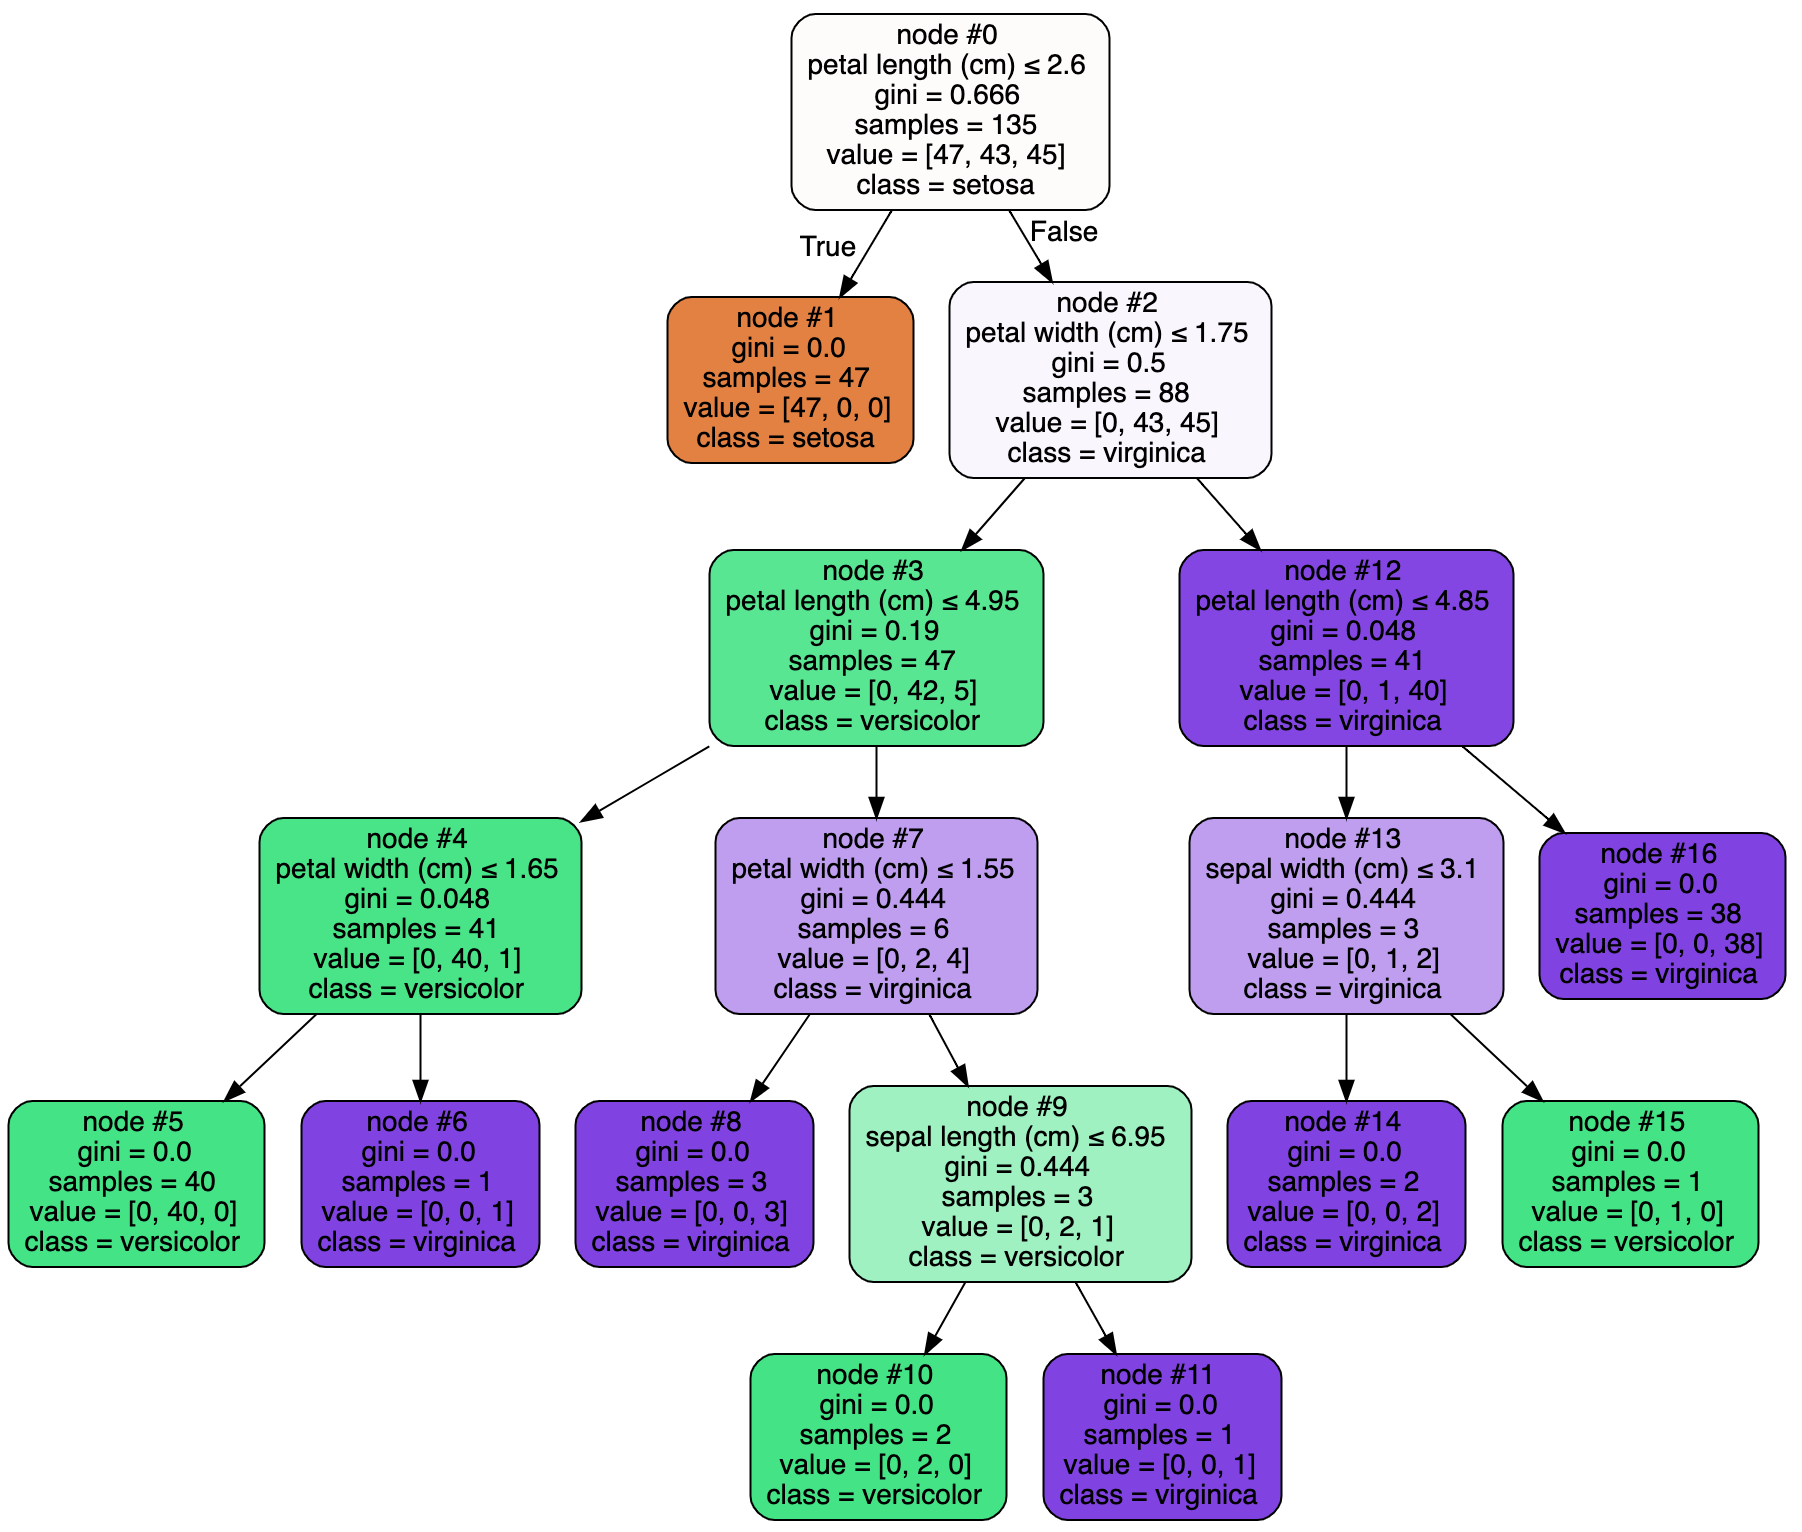
\includegraphics[scale =0.5]{images/Chapter3/decision_tree_model-2609977862.png}
    \caption{A sample decision tree}
    \label{fig:dt}
\end{figure}
An ensemble of many such decision trees result in a `forest' of decision trees which are collectively a `random' forest.

Random forests typically have a number of useful tunable parameters, these parameters are used to both regularize overfitting and improve underfitting.
The most common hyper-parameters that are tuned for random forests are the \texttt{n\_estimators} which are the total number of decision trees in the forest.
A key feature of the random forest is its feature explanability, typically the use of its feature importances, which explain the importance of the different data features in predicting the output of the random forest.
In the example of the Iris species classification, Fig~\ref{fig:RF sample FI} shows the feature importances in predicting the same species as in Fig±\ref{fig:dt}.
The feature importances are relative measures such that the sum of the feature importances is always $1$.
As with the decision tree, the random forest uses multiple features to regress/classify the data and arrive at the desired output.
As it does this process it uses different features, for example in the case of the Iris flower species classification, it uses the petal width as the most important parameter to make this prediction.
This is quite insightful in two ways,
\begin{enumerate}
    \item it is possible to intuit some understanding on the working of the random forest itself by knowing that some features are more relevant to make the desired predictions.
    This is usually the case when we know that the output depends on a few parameters but we are not sure which parameters act as features for the random forest.
    \item it is possible that we have several parameters (as will be the case in my thesis) that could be used to produce the desired output however, we are not sure if this is necessarily true. 
    For example, we have several spectral bins where the absorption lines corresponding to these of an exoplanet are present but we don't know which of these absorption lines allow us to detect and characterize an exoplanet.
\end{enumerate}

Thus, feature importances form the basis to evaluate the features of the data that were learned by the random forest.
This becomes relevant in multiple scenarios, 
\begin{itemize}
    \item when the trained model is overfitting and we can identify and remove those features which produce this overfitting 
    \item when the model is underfitting, the feature importance will allow us to still identify the data features which have a higher relative importance. 
    This can also be problematic because the relative importances can all have very similar values, this is the case when the random forest is not able to fit a generalised model and is the right case for dimensionality reduction
    \item and finally when the model is fitting well and the test and validation accuracies are similar the feature importances are used to study the the features in the data that allow the model to make accurate predictions.
\end{itemize}
\begin{figure}
    \centering
    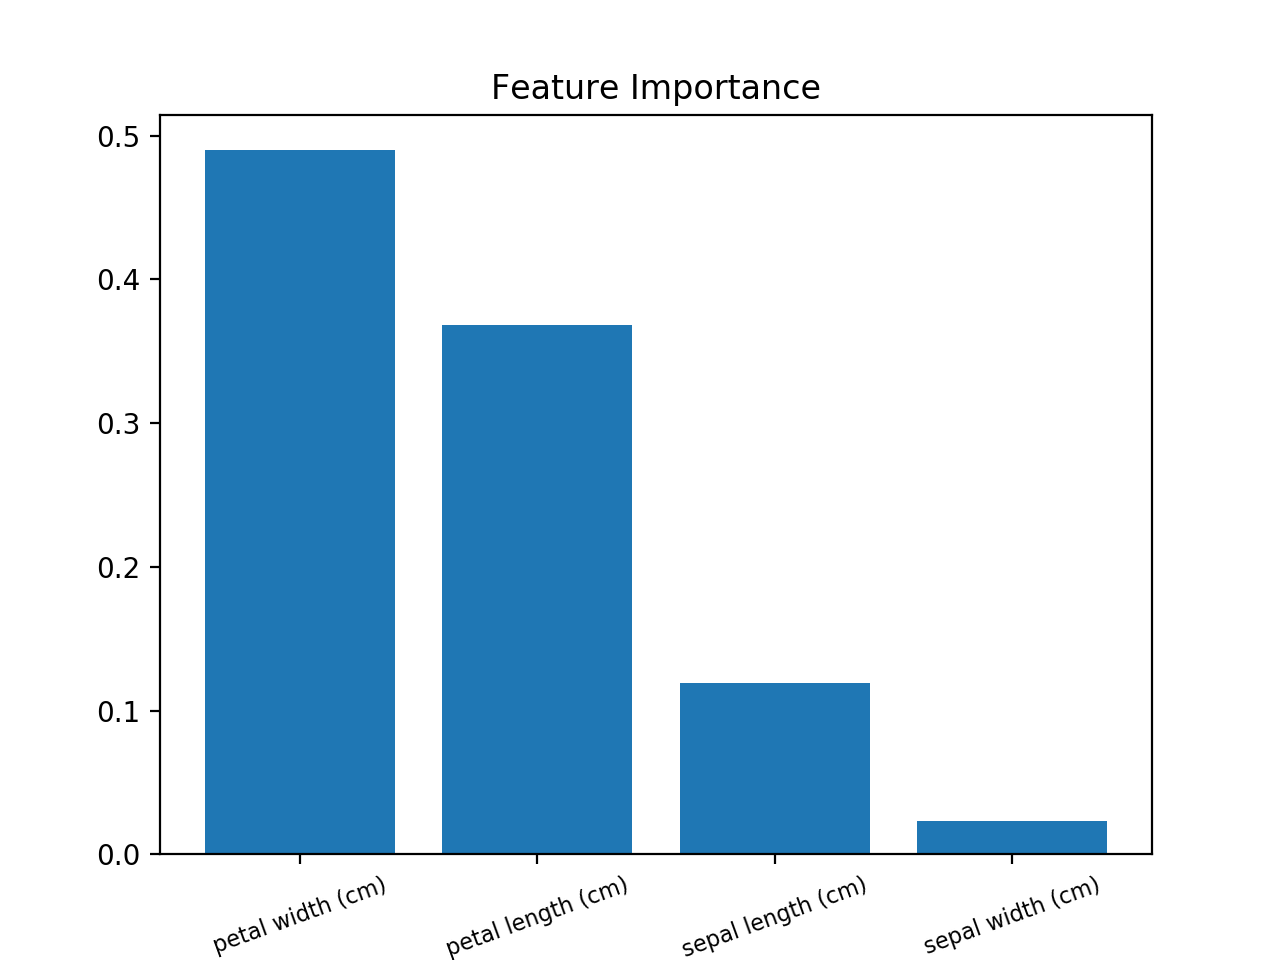
\includegraphics{images/Chapter3/feature_importances_Randomforest.png}
    \caption{RF importances of features used to predict the species of the Iris flower. The y-axis is the relative importance; so a relative importance of $1$ implies the most important and $0$ is the least important feature to predict the species.}
    \label{fig:RF sample FI}
\end{figure}

Random forests are very easily implemented with a two step process with the library \texttt{sklearn} \citep[][]{2011JRFsklearn}.
\section{Multi-layer Perceptrons}
A well known term even amomg non-experts are the words `neural network'.
As the name suggests neural networks are inspired by the network of neurons that make up the mammalian brain.
The basic unit of neural network is a neuron.
A neuron consists of an input, output and an activation function that acts on the input similar to $f(.)$ in Eq~\ref{eq:y=fx}.
This activation function is a mathematical functiom which operates on the input.
Such a unit is called a perceptron and a sample perceptron is depicted in Fig~\ref{fig:perceptron}.
The inputs are combined to form an activation $a_{j}$ via $j$ weights for each input vector value $x_{i}$ making the weight matrix ($w_{ij}$.
The output is defined as ,
\begin{equation}
    y_j = f(\sum_{i=1}^{n} w_{ji}x_i)
    \label{eq: perceptron}
\end{equation}
Many such perceptrons together, producing an output vector $y_{jk}$ for $k$ perceptrons.
This is known as neural network. 
The weights are the neural network parameters whose values can be altered during training.
Activation functions $f(.)$ are typically fixed for the duration of training and varied if the validation results have not reached desirable values.
This is known as a hyper parameter.
The number of neurons in a neural network, the number of weights are also other hyper parameters that can be varied based on the validation results.
The output of a neuron can be treated as an input to another set of perceptrons, and they can be in turn connected to another set of neurons and so on.
Such a network feeds forward the inputs one layer to the next and such networks are called deep neural networks or multi-layer perceptrons.

Based on the kind of combination of $w_{ji}$ and $X_{i}$ perceptron networks can be further sub classified as convolutional neural networks \citep[][]{1990ZhangCNN}, recurrent neural networks and so on.
Neural networks can also work on multi dimensional input as well long vectors.
Configurations of neural networks also vary, for example  other deep neural networks we can also have 

\begin{figure}
    \centering
    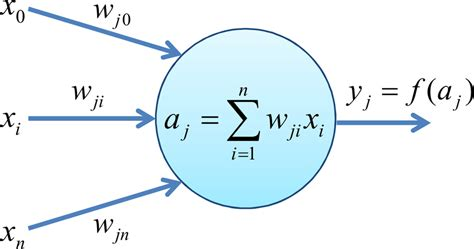
\includegraphics[scale=0.5]{images/Chapter3/perceptron.jpg}
    \caption{A sample percepton consisting of an input vector $X_{i}$ and an output $y$ is depicted here.}
    \label{fig:perceptron}
\end{figure}

\section{Autoencoders}
Autoencoders are special cases of multilayer perceptrons where the input and the output remain fixed but the intermediate layers form a mirrored encoder-decoder structure.
This was first envisioned to denoise data and thus the \citep[denoising autoencoder, ][]{vincent2011connection} was invented.
Typically, the autoencoder has the following main parts,
\begin{itemize}
    \item \textbf{input:} is the input layer which is typically the same shape as the input vector and thus contains as many neurons as the input vector
    \item\textbf{encoder:} the encoder is a set of fully connected neurons which have as input the output of the input layer. 
    These neurons typically are constructed with several layers with the number of neurons in each layer typically reducing in a pyramidal fashion.
    The last layer is the smallest layer and thus the output of this layer is a sparse representation of the input.
    \item\textbf{decoder: } the decoder is a mirror of the encoder both in the layer construction, the number of layers and the neurons used in each layer. 
    It typically terminates in the same number of neurons as the input of the encoder and this layer connects to the output.
    The decoder layer typically reconstructs the input from the sparse representation, thereby recovering a noise free version (note this was the original motivation of the autoencoder).
    \item \textbf{output:} as with the input the output is also a vector equal to the size expected for the output.
\end{itemize}

To wrap this introduction up, we want to make a few points about the limitations of ML algorithms,
\begin{itemize}
    \item \textbf{black box like behavior:} ML algorithms are very useful but also don't particularly lend to great deal of manual fine tuning. 
    Which means that the features that the algorithms learn or not completely controlled and hence to offset this we provide the algorithms with large amount of data.
    \item{\textbf{fine tuning training parameters is challenging:} while there are some thumb rules to follow when training to ensure good training, however there is no way to know if the hyperparameters of the neural network are optimal. 
    Standard techniques such as a parameter space search etc are available but are used when the search itself is not very broad and the parameters have well defined limits}
\end{itemize}
\chapter{Machine learning and astronomy}
\section{Use of deep detection networks}
\section{Applications to exoplanet detection}
\section{Machine learning in direct imaging}
\section{Relevance of using machine learning in simultaneous spectral and imaging targets}